\begin{abstract}
    Digital twins of neutron instruments using Monte Carlo ray tracing have proven to be useful in neutron data analysis and verifying instrument and sample designs. However, these simulations can become quite complex and computationally demanding with tens of billions of neutrons. In this paper, we present a GPU accelerated version of MCViNE using Python and Numba to balance user extensibility with performance. Numba is an open-source just-in-time (JIT) compiler for Python using LLVM to generate efficient machine code for CPUs and GPUs with NVIDIA CUDA. The JIT nature of Numba allowed complex instrument kernels to be generated easily. Initial simulations have shown a speedup between 200-1000x over the original CPU implementation. The performance gain with Numba enables more sophisticated data analysis and impacts neutron scattering science and instrument design.
\end{abstract}

% Adds a frame around verbatim environments
% \fvset{frame=single,fontsize=\footnotesize,samepage=false}

\section{Introduction}

MCViNE \cite{lin2016mcvine,Lin_2019} is a software package for creating digital twins of neutron scattering experiments using a Monte Carlo ray-tracing approach.
In this method, randomly generated probability packets (representing neutrons) are propagated through a series of components.
Each component changes the probability packets according to the physics of the component.
As an example of a component, consider a neutron mirror with less than perfect reflectivity. The interaction between the probability packet and the mirror would cause the velocity component perpendicular to the mirror to reverse and would reduce the probability of the packet to take into account that there is a finite probability that the neutron would not be reflected. The physics of each MCViNE component is documented in the code.
An extensive description of components for a similar package, McStas is provided at \cite{willendrup_components}.
There is no correlation between packets, so the system is embarrassingly parallel.
These simulations are useful in performing advanced neutron data analysis \cite{lin2022super,islam2019super,sala2022ferrimagnetic,do2022damped,leiner2019frustrated,lin2014UN} as well as in designing novel neutron instruments \cite{mamontov2022bwaves,an2022menus,sala2022chess,garlea2022verdi,leighton2022ewald,liu2022pioneer,qian2022centaur,changwoo2022expanse,ankner2023cinematic,hassina2023cupi2d,linjiao2023guide_misalignment} and sample environments \cite{stone2019design,niedziela2017design}. Specifically, it has been used in the initial designs for instruments in the Second Target Station at the Spallation Neutron Source (SNS) \cite{mason2006spallation} at Oak Ridge National Laboratory.
Currently, MCViNE only runs on CPUs which is a bottleneck in large simulations with tens of billions of neutrons, and in modelling complex multiple scattering, with some simulations taking months to complete. Due to the massively parallel nature of Monte Carlo methods, bringing GPU acceleration to these simulations would offer superior performance and scalability. MCViNE was originally implemented in C++ and parallelized using MPI, with bindings to Python for user interaction.
However, extensibility for the end user can be very difficult.

To further improve performance and to create an easily extensible code base, Python and Numba \cite{lam2015numba} were chosen to create a new package of MCViNE providing GPU acceleration, \texttt{mcvine.acc} \cite{Lin_mcvine_acc}. Numba is an open-source JIT (just-in-time) compiler for Python using LLVM to generate efficient machine code and supports GPUs using NVIDIA CUDA. Numba is designed for scientific computing and can support NumPy arrays and functions. Currently, we are only using Numba for its GPU capabilities as the original version of MCViNE is used to run on CPUs. This accelerated MCViNE package is compatible with existing MCViNE scripts, and using a mixture of CPU and GPU components is supported.

This paper will first describe how MCViNE works at a high-level, how components and instruments are created using Numba to generate CUDA kernels, and how Numba is also used to generate kernels for complex sample geometries and scatterers.
Next, we will compare performance of the CPU version of MCViNE to the Numba GPU version.
After that we will describe how the MCViNE GPU acceleration will be used in the larger context of a workflow for data analysis.
Finally, we will discuss our experience using Numba for this application.


\section{Method}

\subsection{MCViNE Overview}

MCViNE simulations are run from a script that defines an instrument, where an instrument is composed of multiple components. A simple 4 component instrument is shown in Figure~\ref{fig:instrument}. Full instruments may have several hundred components. Each instrument script is run with a specified number of probability packets, where each packet has several state variables: position, velocity, spin, probability, and time.

At a high-level, a component takes a neutron as input and performs some action on the neutron. Components can be attached to the instrument at a specified position and orientation. Some of the main component types are sources, guides, monitors, samples, and detectors. In a full instrument simulation, neutrons are generated from a source component and are propagated through each component in the instrument. Sample components are a special type of component with additional input files to specify geometry and material composition.

\begin{figure}[ht]
    \centering
    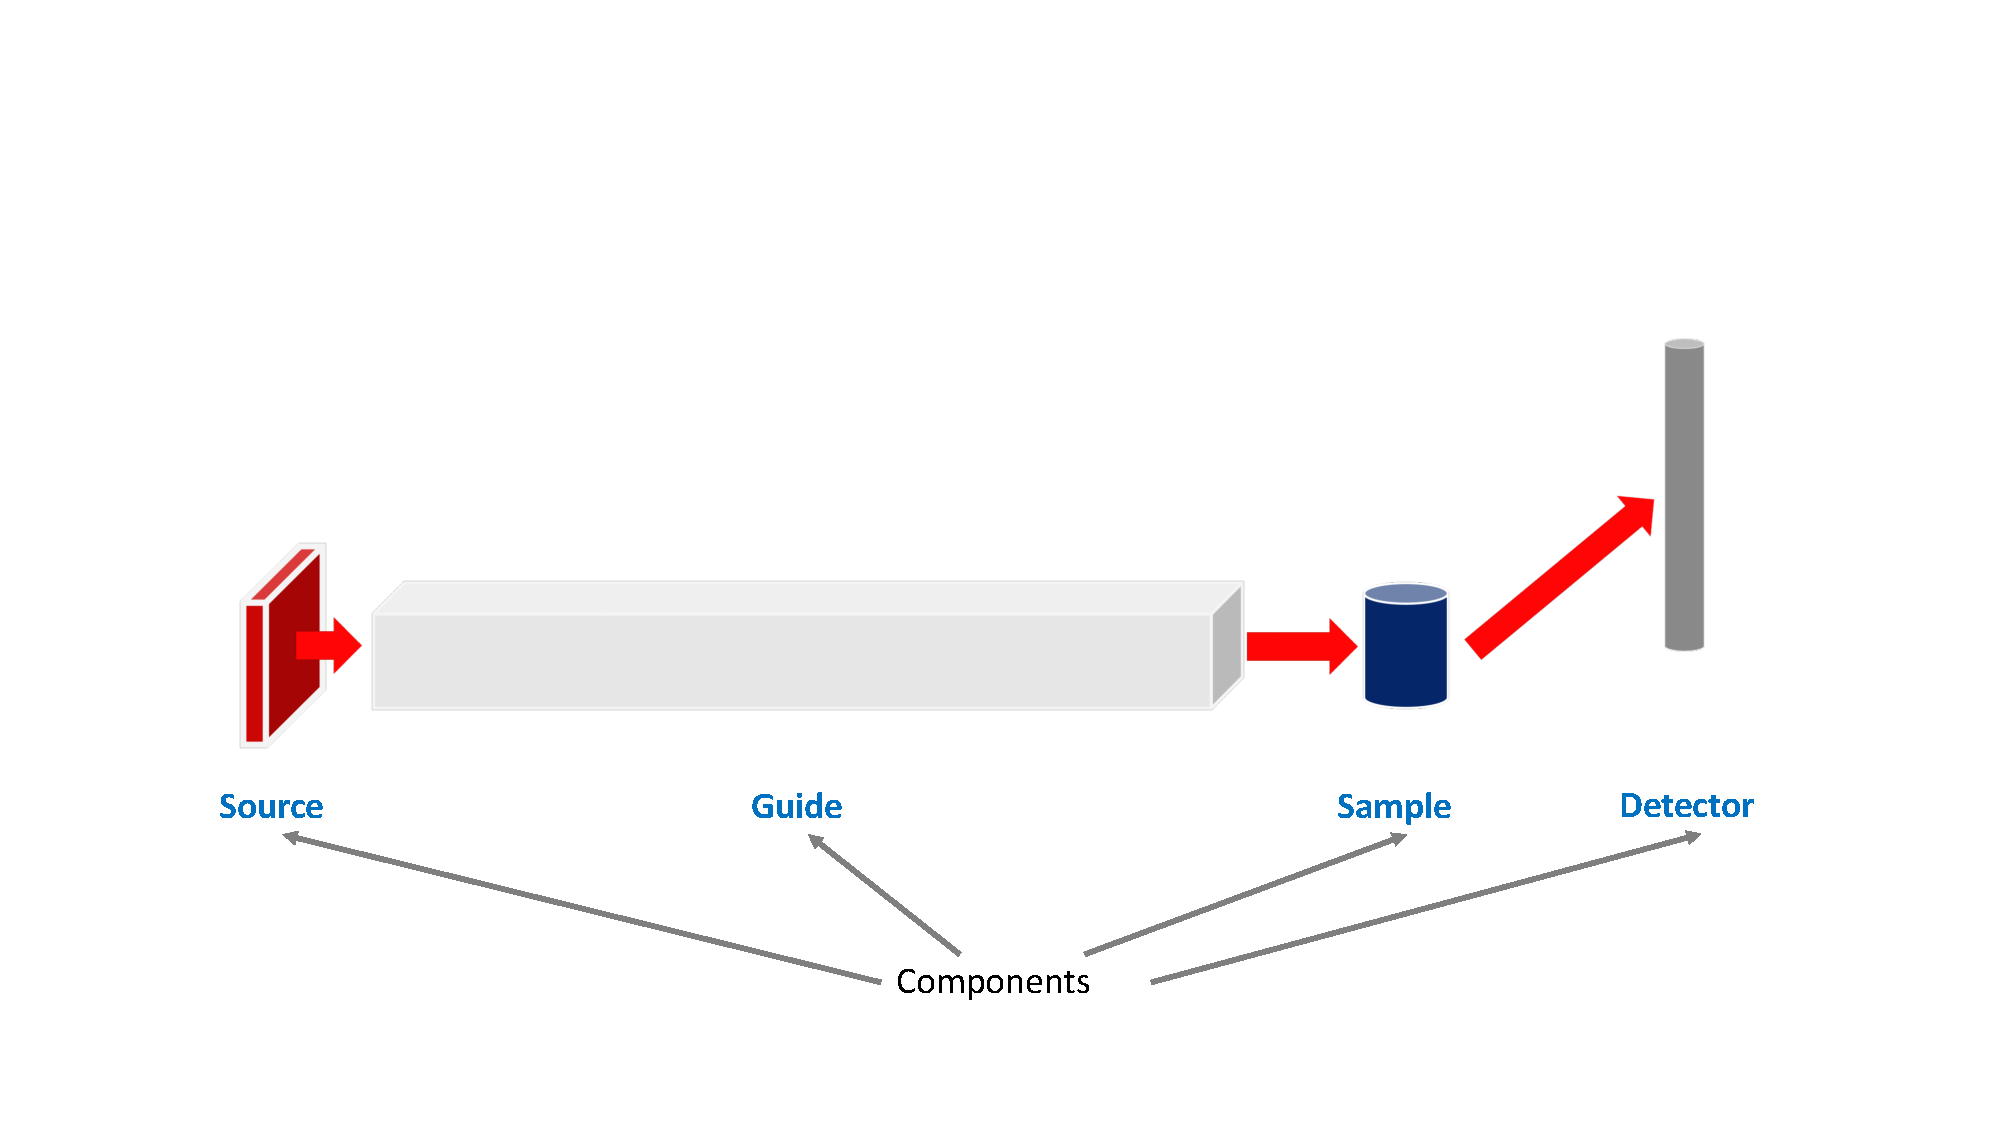
\includegraphics[width=0.45\textwidth, trim={3.5cm 1cm 3.5cm 5cm}, clip]{figures/mcvine_acc_instrument_component_fig.pdf}
    \caption{Example instrument with four components: a source, guide, sample, and detector.}
    \label{fig:instrument}
\end{figure}


\subsection{Component Hierarchy}

One of the major benefits of using Python for this application is the ease of utilizing an object-oriented design and polymorphism.
Each component inherits from a base \texttt{AbstractComponent} class. This \texttt{AbstractComponent} class requires a ``propagate'' method to be defined which takes in a neutron for the first parameter. The ``propagate'' method is responsible for defining the action of the component and is decorated with \texttt{@cudajit} to indicate that it is a CUDA kernel. An example of creating a simple component can be seen below. Additional parameters can be specified, but must also be defined in the \texttt{propagate\_params} list.
There are several major types of components that have their own subclasses: \texttt{SampleBase}, \texttt{SourceBase}, and \texttt{MonitorBase}.

\vspace{1mm}
\begin{Verbatim}[commandchars=\\\{\}]
\PY{k+kn}{from} \PY{n+nn}{mcvine.acc.ComponentBase} \PY{k+kn}{import} \PY{n}{ComponentBase}
\PY{k}{class} \PY{n+nc}{Arm}\PY{p}{(}\PY{n}{ComponentBase}\PY{p}{)}\PY{p}{:}

    \PY{k}{def} \PY{n+nf+fm}{\PYZus{}\PYZus{}init\PYZus{}\PYZus{}}\PY{p}{(}\PY{n+nb+bp}{self}\PY{p}{,} \PY{n}{name}\PY{p}{,} \PY{o}{*}\PY{o}{*}\PY{n}{kwargs}\PY{p}{)}\PY{p}{:}
        \PY{n+nb+bp}{self}\PY{o}{.}\PY{n}{name} \PY{o}{=} \PY{n}{name}
        \PY{n+nb+bp}{self}\PY{o}{.}\PY{n}{propagate\PYZus{}params} \PY{o}{=} \PY{p}{(}\PY{p}{)}

        \PY{c+c1}{\PYZsh{} Aim a neutron at this arm to }
        \PY{c+c1}{\PYZsh{} cause JIT compilation.}
        \PY{k+kn}{import} \PY{n+nn}{mcni}
        \PY{n}{neutrons} \PY{o}{=} \PY{n}{mcni}\PY{o}{.}\PY{n}{neutron\PYZus{}buffer}\PY{p}{(}\PY{l+m+mi}{1}\PY{p}{)}
        \PY{n}{neutrons}\PY{p}{[}\PY{l+m+mi}{0}\PY{p}{]} \PY{o}{=} \PYZbs{}
            \PY{n}{mcni}\PY{o}{.}\PY{n}{neutron}\PY{p}{(}\PY{n}{r}\PY{o}{=}\PY{p}{(}\PY{l+m+mi}{0}\PY{p}{,} \PY{l+m+mi}{0}\PY{p}{,} \PY{o}{\PYZhy{}}\PY{l+m+mi}{1}\PY{p}{)}\PY{p}{,} 
                         \PY{n}{v}\PY{o}{=}\PY{p}{(}\PY{l+m+mi}{0}\PY{p}{,} \PY{l+m+mi}{0}\PY{p}{,} \PY{l+m+mi}{1}\PY{p}{)}\PY{p}{,} 
                         \PY{n}{prob}\PY{o}{=}\PY{l+m+mi}{1}\PY{p}{,} \PY{n}{time}\PY{o}{=}\PY{l+m+mi}{0}\PY{p}{)}
        \PY{n+nb+bp}{self}\PY{o}{.}\PY{n}{process}\PY{p}{(}\PY{n}{neutrons}\PY{p}{)}

    \PY{n+nd}{@cuda.jit}\PY{p}{(}\PY{n}{void}\PY{p}{(}\PY{n}{NB\PYZus{}FLOAT}\PY{p}{[}\PY{p}{:}\PY{p}{]}\PY{p}{)}\PY{p}{,} 
              \PY{n}{device}\PY{o}{=}\PY{n+nb+bp}{True}\PY{p}{)}
    \PY{k}{def} \PY{n+nf}{propagate}\PY{p}{(}\PY{n}{in\PYZus{}neutron}\PY{p}{)}\PY{p}{:}
        \PY{k}{pass}
\end{Verbatim}


\subsection{CUDA Kernel Generation for an Instrument}

In order to run a simulation from an input instrument script, \texttt{mcvine.acc} first generates a GPU kernel from the instrument specification. The input script will be parsed and then ``compiled'' to generate a Python script representing an instrument kernel. This compiled version is then imported and executed to run the simulation. An example of a simple MCViNE instrument script containing a source, guide, and monitor can be seen below.

\vspace{1mm}
\begin{lstlisting}[language=python]
def instrument():
    instrument = mcvine.instrument()
    source = Source_simple(
        'src',
        radius = 0., width = 0.03,
        height = 0.03, dist = 1.,
        xw = 0.035, yh = 0.035
    )
    instrument.append(source,
                      position=(0,0,0.))

    guide1 = Guide(
        'guide',
        w1=0.035, h1=0.035,
        w2=0.035, h2=0.035,
        l=10
    )
    instrument.append(guide1,
                      position=(0,0,1.))

    mon = PosDiv_monitor(
        'mon', xwidth=0.08, yheight=0.08,
        maxdiv=2.,
        npos=250, ndiv=251,
    )
    instrument.append(mon,
                      position=(0,0,12.))
    return instrument
\end{lstlisting}

\vspace{1mm}

When \texttt{mcvine.acc} is called on the above instrument script, a new Python file is generated which contains a Numba CUDA kernel for the entire instrument. Each of the instrument components' \texttt{process} kernels are collected and inserted to form a generic kernel in this process. This generated kernel effectively models a neutron travelling through the entire instrument.

Depending on the kernel launch configuration, each GPU thread might be responsible for more than one neutron. An example of a compiled instrument script can be seen in the code listing below. As seen in the script, a CUDA kernel is defined using Numba. Inside the kernel, each GPU thread will loop over the number of neutrons it is processing. Each \texttt{propagate} function has a number appended to it. These propagate functions correspond to the Component's propagate method. For this case, \texttt{propagate0} matches the Source component propagate kernel, \texttt{propagate1} matches the Guide component propagate kernel, and so on. The \texttt{applyTransformation} function is inserted in-between instrument components and is responsible for translating the position/velocity of a neutron in the current component's coordinate system to that of the next component by applying a transformation matrix.

\vspace{1mm}
\begin{Verbatim}[commandchars=\\\{\},fontsize=\tiny]
\PY{n+nd}{@cuda.jit}
\PY{k}{def} \PY{n+nf}{process\PYZus{}kernel\PYZus{}no\PYZus{}buffer}\PY{p}{(}
    \PY{n}{rng\PYZus{}states}\PY{p}{,} \PY{n}{N}\PY{p}{,} \PY{n}{n\PYZus{}neutrons\PYZus{}per\PYZus{}thread}\PY{p}{,}
    \PY{n}{args}
\PY{p}{)}\PY{p}{:}
    \PY{n}{args0}\PY{p}{,} \PY{n}{args1}\PY{p}{,} \PY{n}{args2}\PY{p}{,} \PY{n}{offsets}\PY{p}{,} \PY{n}{rotmats}\PY{p}{,} \PY{n}{neutron\PYZus{}counter} \PY{o}{=} \PY{n}{args}
    \PY{n}{thread\PYZus{}index} \PY{o}{=} \PY{n}{cuda}\PY{o}{.}\PY{n}{grid}\PY{p}{(}\PY{l+m+mi}{1}\PY{p}{)}
    \PY{n}{start\PYZus{}index} \PY{o}{=} \PY{n}{thread\PYZus{}index}\PY{o}{*}\PY{n}{n\PYZus{}neutrons\PYZus{}per\PYZus{}thread}
    \PY{n}{end\PYZus{}index} \PY{o}{=} \PY{n+nb}{min}\PY{p}{(}\PY{n}{start\PYZus{}index}\PY{o}{+}\PY{n}{n\PYZus{}neutrons\PYZus{}per\PYZus{}thread}\PY{p}{,} \PY{n}{N}\PY{p}{)}
    \PY{n}{neutron} \PY{o}{=} \PY{n}{cuda}\PY{o}{.}\PY{n}{local}\PY{o}{.}\PY{n}{array}\PY{p}{(}\PY{n}{shape}\PY{o}{=}\PY{l+m+mi}{10}\PY{p}{,} \PY{n}{dtype}\PY{o}{=}\PY{n}{NB\PYZus{}FLOAT}\PY{p}{)}
    \PY{n}{r} \PY{o}{=} \PY{n}{cuda}\PY{o}{.}\PY{n}{local}\PY{o}{.}\PY{n}{array}\PY{p}{(}\PY{l+m+mi}{3}\PY{p}{,} \PY{n}{dtype}\PY{o}{=}\PY{n}{NB\PYZus{}FLOAT}\PY{p}{)}
    \PY{n}{v} \PY{o}{=} \PY{n}{cuda}\PY{o}{.}\PY{n}{local}\PY{o}{.}\PY{n}{array}\PY{p}{(}\PY{l+m+mi}{3}\PY{p}{,} \PY{n}{dtype}\PY{o}{=}\PY{n}{NB\PYZus{}FLOAT}\PY{p}{)}
    \PY{k}{for} \PY{n}{neutron\PYZus{}index} \PY{o+ow}{in} \PY{n+nb}{range}\PY{p}{(}\PY{n}{start\PYZus{}index}\PY{p}{,} \PY{n}{end\PYZus{}index}\PY{p}{)}\PY{p}{:}
        \PY{n}{cuda}\PY{o}{.}\PY{n}{atomic}\PY{o}{.}\PY{n}{add}\PY{p}{(}\PY{n}{neutron\PYZus{}counter}\PY{p}{,} \PY{l+m+mi}{0}\PY{p}{,} \PY{l+m+mi}{1}\PY{p}{)}
        \PY{n}{propagate0}\PY{p}{(}\PY{n}{thread\PYZus{}index}\PY{p}{,} \PY{n}{rng\PYZus{}states}\PY{p}{,}  \PY{n}{neutron}\PY{p}{,} \PY{o}{*}\PY{n}{args0}\PY{p}{)}
        \PY{n}{applyTransformation}\PY{p}{(}\PY{n}{neutron}\PY{p}{[}\PY{p}{:}\PY{l+m+mi}{3}\PY{p}{]}\PY{p}{,} \PY{n}{neutron}\PY{p}{[}\PY{l+m+mi}{3}\PY{p}{:}\PY{l+m+mi}{6}\PY{p}{]}\PY{p}{,} 
                            \PY{n}{rotmats}\PY{p}{[}\PY{l+m+mi}{0}\PY{p}{]}\PY{p}{,} \PY{n}{offsets}\PY{p}{[}\PY{l+m+mi}{0}\PY{p}{]}\PY{p}{,} \PY{n}{r}\PY{p}{,} \PY{n}{v}\PY{p}{)}
        \PY{n}{propagate1}\PY{p}{(}\PY{n}{neutron}\PY{p}{,} \PY{o}{*}\PY{n}{args1}\PY{p}{)}
        \PY{n}{applyTransformation}\PY{p}{(}\PY{n}{neutron}\PY{p}{[}\PY{p}{:}\PY{l+m+mi}{3}\PY{p}{]}\PY{p}{,} \PY{n}{neutron}\PY{p}{[}\PY{l+m+mi}{3}\PY{p}{:}\PY{l+m+mi}{6}\PY{p}{]}\PY{p}{,} 
                            \PY{n}{rotmats}\PY{p}{[}\PY{l+m+mi}{1}\PY{p}{]}\PY{p}{,} \PY{n}{offsets}\PY{p}{[}\PY{l+m+mi}{1}\PY{p}{]}\PY{p}{,} \PY{n}{r}\PY{p}{,} \PY{n}{v}\PY{p}{)}
        \PY{n}{propagate2}\PY{p}{(}\PY{n}{neutron}\PY{p}{,} \PY{o}{*}\PY{n}{args2}\PY{p}{)}

\PY{k+kn}{from} \PY{n+nn}{mcvine.acc.components.sources.SourceBase} \PY{k+kn}{import} \PY{n}{SourceBase}
\PY{k}{class} \PY{n+nc}{\PYZus{}Base}\PY{p}{(}\PY{n}{SourceBase}\PY{p}{)}\PY{p}{:} \PY{c+c1}{\PYZsh{} has to be named Base in definition}
    \PY{k}{def} \PY{n+nf+fm}{\PYZus{}\PYZus{}init\PYZus{}\PYZus{}}\PY{p}{(}\PY{n+nb+bp}{self}\PY{p}{,} \PY{n}{instrument}\PY{p}{)}\PY{p}{:}
        \PY{n}{offsets}\PY{p}{,} \PY{n}{rotmats} \PY{o}{=} \PY{n}{calcTransformations}\PY{p}{(}\PY{n}{instrument}\PY{p}{)}
        \PY{n+nb+bp}{self}\PY{o}{.}\PY{n}{neutron\PYZus{}counter} \PY{o}{=} \PY{n}{neutron\PYZus{}counter} \PY{o}{=} \PY{n}{np}\PY{o}{.}\PY{n}{zeros}\PY{p}{(}\PY{l+m+mi}{1}\PY{p}{,} \PY{n}{dtype}\PY{o}{=}\PY{n+nb}{int}\PY{p}{)}
        \PY{n+nb+bp}{self}\PY{o}{.}\PY{n}{propagate\PYZus{}params} \PY{o}{=} \PY{n+nb}{tuple}\PY{p}{(}
            \PY{n}{c}\PY{o}{.}\PY{n}{propagate\PYZus{}params} \PY{k}{for} \PY{n}{c} \PY{o+ow}{in} \PY{n}{instrument}\PY{o}{.}\PY{n}{components}\PY{p}{)}
        \PY{n+nb+bp}{self}\PY{o}{.}\PY{n}{propagate\PYZus{}params} \PY{o}{+}\PY{o}{=} \PY{p}{(}\PY{n}{offsets}\PY{p}{,} \PY{n}{rotmats}\PY{p}{,} \PY{n}{neutron\PYZus{}counter}\PY{p}{)}
        \PY{k}{return}
    \PY{k}{def} \PY{n+nf}{propagate}\PY{p}{(}\PY{n+nb+bp}{self}\PY{p}{)}\PY{p}{:} \PY{k}{return}
\PY{n}{InstrumentWrapper} \PY{o}{=} \PY{n}{\PYZus{}Base}
\PY{n}{InstrumentWrapper}\PY{o}{.}\PY{n}{process\PYZus{}kernel\PYZus{}no\PYZus{}buffer} \PY{o}{=} \PY{n}{process\PYZus{}kernel\PYZus{}no\PYZus{}buffer}

\PY{k}{def} \PY{n+nf}{run}\PY{p}{(}\PY{n}{ncount}\PY{p}{,} \PY{n}{ntotalthreads}\PY{o}{=}\PY{n+nb+bp}{None}\PY{p}{,} \PY{n}{threads\PYZus{}per\PYZus{}block}\PY{o}{=}\PY{n+nb+bp}{None}\PY{p}{,} \PY{o}{*}\PY{o}{*}\PY{n}{kwds}\PY{p}{)}\PY{p}{:}
    \PY{n}{instrument} \PY{o}{=} \PY{n}{loadInstrument}\PY{p}{(}\PY{n}{script}\PY{p}{,} \PY{o}{*}\PY{o}{*}\PY{n}{kwds}\PY{p}{)}
    \PY{n}{iw} \PY{o}{=} \PY{n}{InstrumentWrapper}\PY{p}{(}\PY{n}{instrument}\PY{p}{)}
    \PY{n}{iw}\PY{o}{.}\PY{n}{process\PYZus{}no\PYZus{}buffer}\PY{p}{(}\PY{n}{ncount}\PY{p}{,} \PY{n}{ntotalthreads}\PY{o}{=}\PY{n}{ntotalthreads}\PY{p}{,}
                         \PY{n}{threads\PYZus{}per\PYZus{}block}\PY{o}{=}\PY{n}{threads\PYZus{}per\PYZus{}block}\PY{p}{)}
    \PY{n}{processed} \PY{o}{=} \PY{n}{iw}\PY{o}{.}\PY{n}{neutron\PYZus{}counter}\PY{p}{[}\PY{l+m+mi}{0}\PY{p}{]}
    \PY{n}{saveMonitorOutputs}\PY{p}{(}\PY{n}{instrument}\PY{p}{,} \PY{n}{scale\PYZus{}factor}\PY{o}{=}\PY{l+m+mf}{1.0}\PY{o}{/}\PY{n}{ncount}\PY{p}{)}
\end{Verbatim}

\vspace{1mm}

\subsection{Sample Kernels and CSG}

One unique feature of MCViNE is its sample component, which allows for simulation of complex sample/sample environment and detector systems with flexible, sophisticated geometry and scattering physics.
This feature has enabled simulations that produce virtual experiment data that closely resemble real experimental data and make MCViNE a useful tool for both instrument design and advanced data analysis.

A Sample is made up of a Sample Assembly which has \texttt{Shape} and \texttt{Phase} tags.
The \texttt{Shape} tag contains the geometry specification. The \texttt{Phase} tag, together with additional XML file(s) named \texttt{\{name\}-scatterer.xml}, contain the scattering physics specification where \texttt{\{name\}} is the name of a scatterer included in the sample assembly.
A simple example for an aluminum (Al) sphere is shown below.
Such an Al sphere is an idealized sample, where the sphere matches the scattering condition and Al is the material most transparent to neutron and is used for mounts and sample containers. Therefore it is well studied and well understood.

\vspace{1mm}
\begin{lstlisting}[language=python]
<?xml version="1.0"?>

<!DOCTYPE SampleAssembly>

<SampleAssembly name="isotropic_sphere">
  <PowderSample name="sample" type="sample">
    <Shape>
      <sphere radius="1*cm" />
    </Shape>
    <Phase type="crystal">
      <ChemicalFormula>Al</ChemicalFormula>
      <xyzfile>Al.xyz</xyzfile>
    </Phase>
  </PowderSample>
  <LocalGeometer registry-coordinate-system="InstrumentScientist">
    <Register name="sample" position="(0,0,0)" orientation="(0,0,0)"/>
  </LocalGeometer>
</SampleAssembly>
\end{lstlisting}

\vspace{1mm}

Simple shapes can be created easily, but more complex shapes can be created too.
To create the sample geometry, MCViNE uses Constructive Solid Geometry (CSG).
CSG can create complex geometries from operations such as intersection and union, on primitive shapes, such as cubes, spheres, and cylinders.
For example, Figure~\ref{fig:csg} shows how CSG is used to create an annular sample can from cylindrical primitives. This can is similar to those used in experiment design \cite{PhysRevB.107.094511}.
First a ring for the outside of the can is made from two cylinders by subtraction, then a ring for the inside of the can is also made from two cylinders.  These two rings are then combined in union with another cylinder that is the bottom of the can.

\begin{figure}[h]
    \centering
    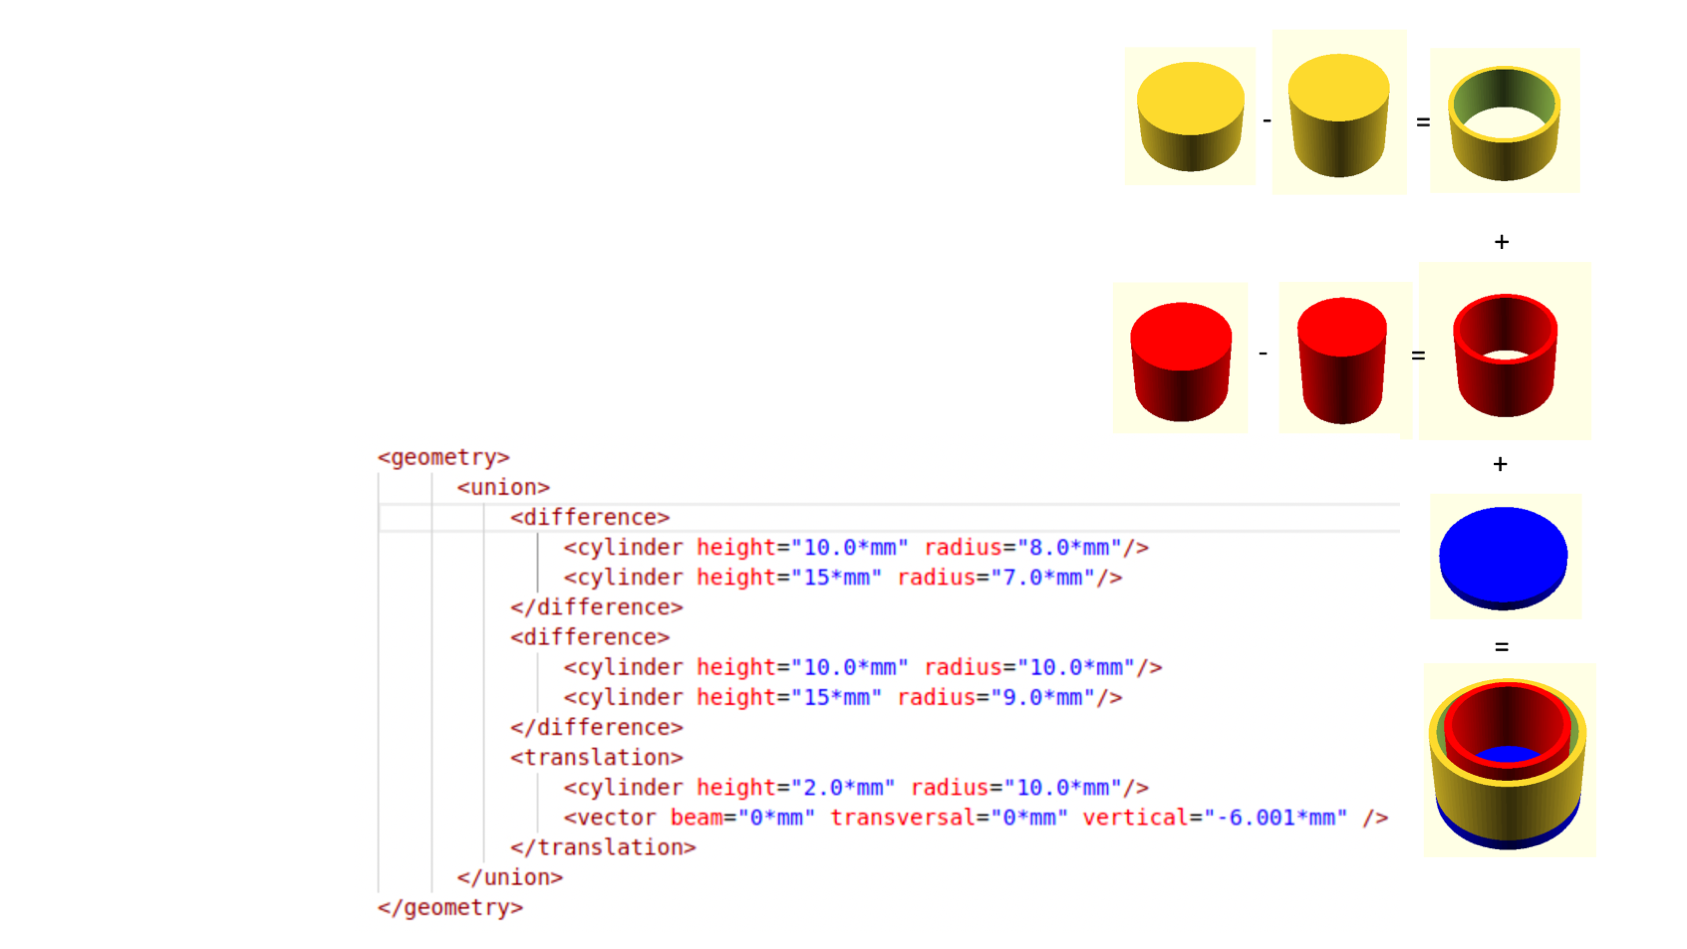
\includegraphics[trim = {1.2cm 0 4cm 0 }, width=\columnwidth]{figures/mcvine_CSG_example.png}
    \caption{An example of an annular sample can  created using CSG (right) and how the primitives and operations are specified in XML as input to MCViNE.}
    \label{fig:csg}
\end{figure}

Ray tracing routines are implemented as CUDA kernels for these primitive shapes and operations. To support complex geometries that might involve many operations and shapes, the visitor pattern is used which constructs a single CUDA kernel to handle the ray intersection of that shape. This highlights one of the major advantages of using Python and Numba, as the ability to generate a CUDA kernel dynamically at run-time would be much more difficult to implement in other languages.

The specification of the scattering physics of a particular neutron scatterer is described in a dedicated ``scatterer'' XML file, where one or more sample kernels can be specified.
An example of a scatterer XML file for specifying scattering physics can be seen below.

\vspace{1mm}
\begin{Verbatim}[commandchars=\\\{\},fontsize=\tiny]
\PY{c+cp}{\PYZlt{}?xml version=\PYZdq{}1.0\PYZdq{}?\PYZgt{}}

\PY{c+cp}{\PYZlt{}!DOCTYPE scatterer\PYZgt{}}

\PY{c}{\PYZlt{}!\PYZhy{}\PYZhy{}}\PY{c}{ weights: absorption, scattering, transmission }\PY{c}{\PYZhy{}\PYZhy{}\PYZgt{}}
\PY{n+nt}{\PYZlt{}homogeneous\PYZus{}scatterer} \PY{n+na}{mcweights=}\PY{l+s}{\PYZdq{}0, 1, 0\PYZdq{}}\PY{n+nt}{\PYZgt{}}
  \PY{n+nt}{\PYZlt{}IsotropicKernel} \PY{n+na}{absorption\PYZus{}coefficient=}\PY{l+s}{\PYZdq{}10./m\PYZdq{}} \PY{n+na}{scattering\PYZus{}coefficient=}\PY{l+s}{\PYZdq{}10./m\PYZdq{}}\PY{n+nt}{\PYZgt{}}
  \PY{n+nt}{\PYZlt{}/IsotropicKernel\PYZgt{}}
\PY{n+nt}{\PYZlt{}/homogeneous\PYZus{}scatterer\PYZgt{}}
\end{Verbatim}

\vspace{1mm}

Note the format is extensible enough to allow a composite scatterer with multiple scatters, though at the time of writing this paper the Numba version of this functionality is still under development.


\section{Results}

Two types of comparisons were performed to show the usefulness of \texttt{mcvine.acc}. First, simulations comparing the CPU and GPU shows a significant performance gain by using a GPU (Figures~\ref{fig:results_isotropic_sphere} -- \ref{fig:results_ms}).
Second, simulations from a more complete instrument solution showing equivalent outcomes from a CPU and GPU simulation were performed (Figure~\ref{fig:UN_plot} and~\ref{fig:UN_cuts}).

\begin{figure}[h]
    \centering
    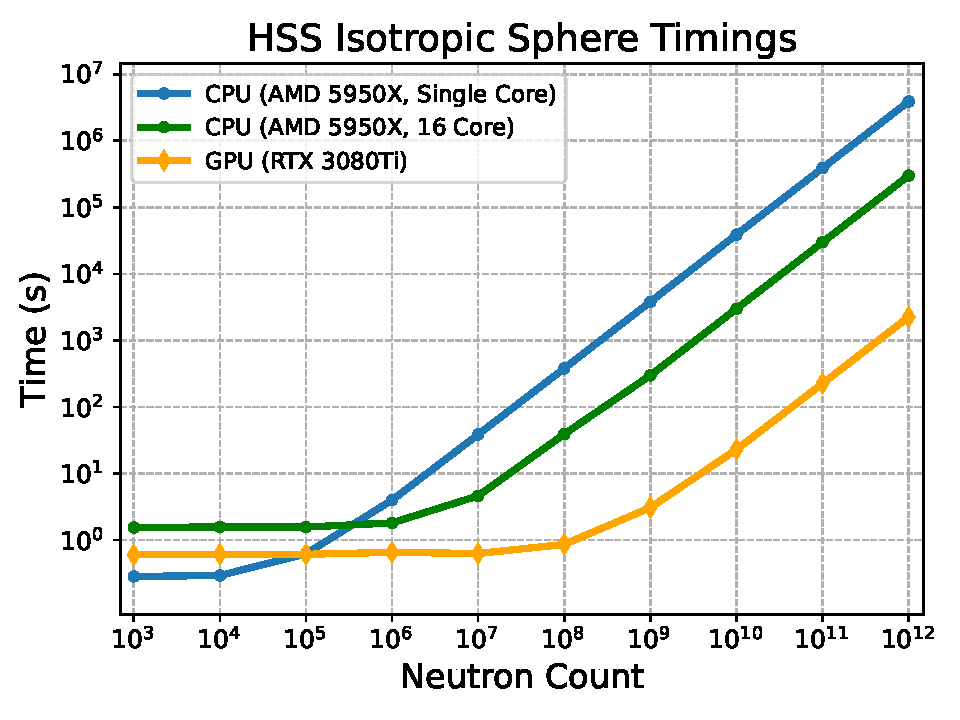
\includegraphics[width=\columnwidth]{figures/mcvine_hss_isotropic_timings.pdf}
    \caption{Time versus neutron counts for  a single core CPU (blue line), multi-core CPU (green line), and GPU (orange line) for a simple instrument using a homogeneous single scatterer (HSS) with a aluminum sphere sample.}
    \label{fig:results_isotropic_sphere}
\end{figure}

For the first study, we focus on the performance gain achieved by the GPU accelerated version of MCViNE.
We used a simple instrument consisting of a source, sample, and detector to focus on the sample assembly component.
We performed tests with two different samples: a simple spherical sample with an isotropic scattering kernel, and a second with a more complex Uranium Nitride (UN) sample.
The UN sample was chosen as it has been experimentally studied and is well modeled by single and multiple scattering of a Quantum Harmonic oscillator model \cite{aczel2012quantum,lin2014UN}.
The UN sample is treated as a 1 cm polycrystalline cube to match the experimental configuration \cite{aczel2012quantum}.
The UN structure is the same as  rock salt structure with the light N atoms located between the much heavier U atoms.
The N vibrates as a harmonic oscillator which provides equally spaced lines in energy transfer $E$.
The lines are modeled in MCViNE with a sample scattering kernel containing a composite of $E(Q)$ kernels with constant $E$ values of a 50 meV spacing from 0 to 350 meV.

Figure~\ref{fig:results_isotropic_sphere} shows the performance of the isotropic sphere sample for the CPU version of MCViNE with one and 16 cores (blue and green curves) compared to the GPU version of MCViNE (orange curve). At $10^{12}$ neutrons, \texttt{mcvine.acc} achieves a speedup of 1725x over a single core and 133x over 16 cores.


Two versions of this simulation were run for the UN sample: the first with only single scattering events (Figure~\ref{fig:results_ss}), and the second with single and multiple scattering events (Figure~\ref{fig:results_ms}).
Single scattering was implemented first to verify the overall workflow and kernel generation of \texttt{mcvine.acc}. Multiple scattering was then added to fully capture the realistic scattering physics.
Multiple scattering is much more computationally intensive since each neutron can scatter more than once.

\begin{figure}[h]
    \centering
    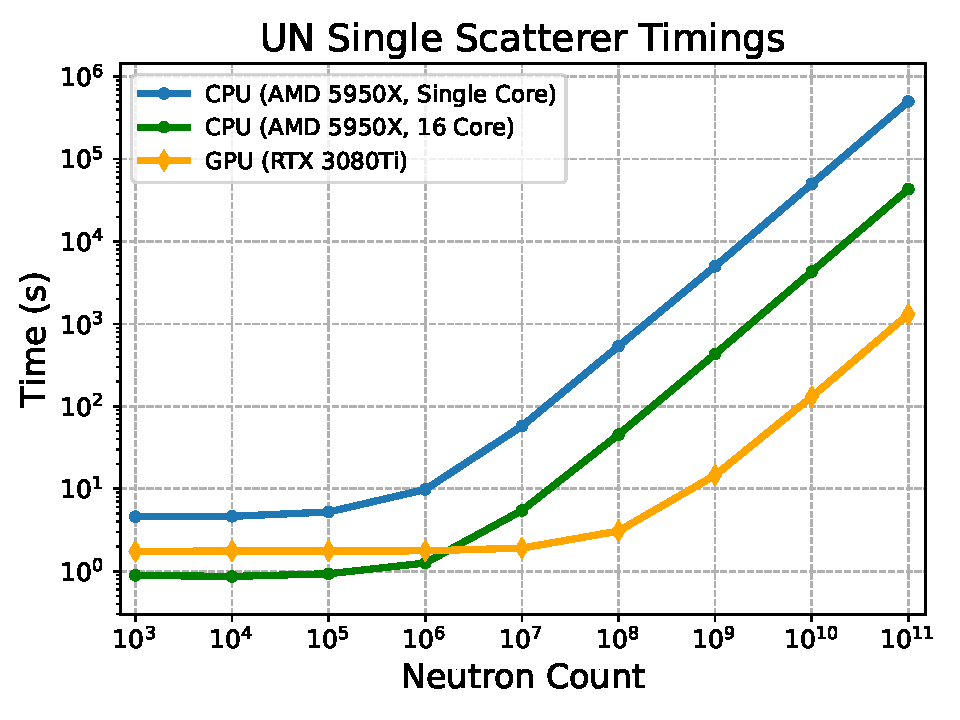
\includegraphics[width=\columnwidth]{figures/mcvine_un_ss_timings.pdf}
    \caption{Time versus neutron counts for a single core CPU (blue line), multi-core CPU (green line), and GPU (orange line) and GPU (orange line) for the UN instrument with single scattering.}
    \label{fig:results_ss}
\end{figure}

\begin{figure}[h]
    \centering
    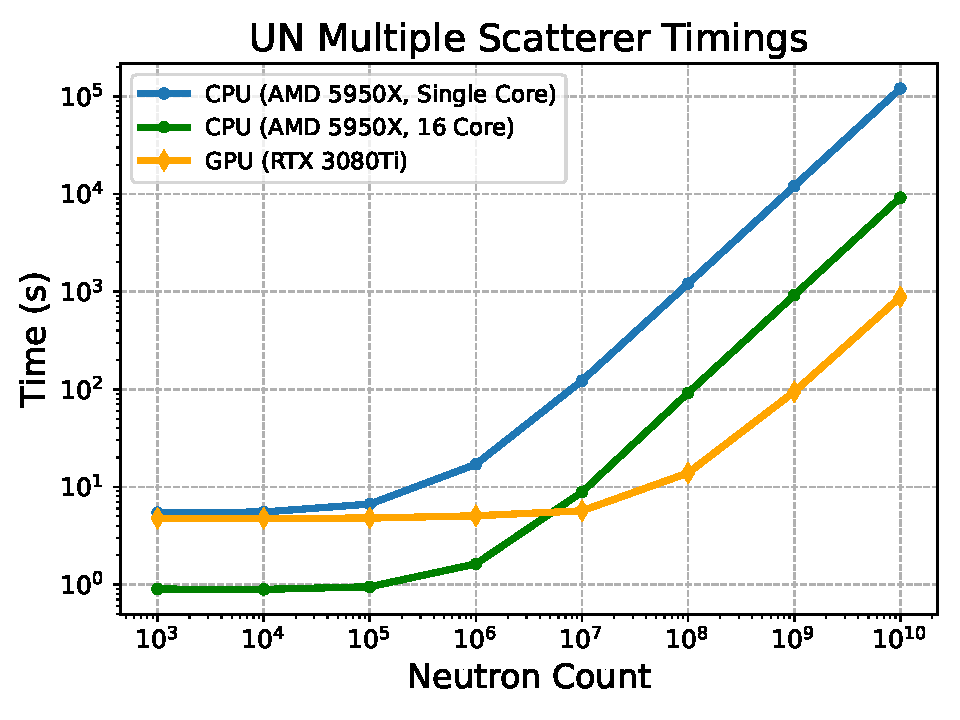
\includegraphics[width=\columnwidth]{figures/mcvine_un_ms_timings.pdf}
    \caption{Time versus neutron counts for a single core CPU (blue line), multi-core CPU (green line), and GPU (orange line) for the UN instrument with multiple scattering.}
    \label{fig:results_ms}
\end{figure}


\begin{table}[h]
    \centering
    \begin{tabular}{c|c|c}
        Simulation Type & Speedup over 1 Core & Speedup over 16 Cores \\
        \hline
        HSS Isotropic Sphere & 1725 & 133 \\
        UN Single Scatterer & 383 & 33 \\
        UN Multiple Scatterer & 137 & 10 \\
        \hline
    \end{tabular}
    \caption{Speedup achieved by \texttt{mcvine.acc} over the CPU with one core and 16 cores for each type of simulation.}
    \label{tab:speedup}
\end{table}


For the UN single scattering case, Figure~\ref{fig:results_ss} shows that for $10^{11}$ neutrons, the GPU version obtained a speedup of 383x over a single core, and 33x over 16 cores. For the UN multiple scattering case, Figure~\ref{fig:results_ms} shows that for $10^{10}$ neutrons, the GPU version obtained a speedup of 137x over a single core, and 10x over 16 cores. Comparing the speedup achieved for the simple isotropic sphere to the UN with single and multiple scattering shows the additional complexity required for the UN sample. A speedup of 10x over 16-core CPU for the UN multiple scattering case is still significant as some simulations can take on the order of days to months to complete.

While the speedup over the CPU version of MCViNE is significant, further optimization is possible. Currently, each GPU thread executes a single large kernel that models the instrument. For large instruments that contain many components, the instrument kernel can use too many registers which limits device occupancy. Additionally, a lot of components involve many conditional statements which do not perform well on the GPU. This can be seen by comparing the performance of complex sample components, such as the UN sample, to the simple isotropic sphere.

Next we run a more complete test with the Uranium Nitride sample to verify the same result between the CPU and GPU.
A study on UN was the first time the multiple-scattering as well as the multiple-scattering physics in the CPU version of MCViNE was used to explain experimental results \cite{lin2014UN}. Specifically, one of the puzzles from the measured data was that the equally spaced lines extend over all $Q$.  It was determined that this was due to multiple scattering.
To more conclusively check this, a CPU simulation using MCViNE was performed \cite{lin2014UN}.  At the time this CPU simulation was run, it took days to do such calculations.  Therefore, this is a good test case to check the speed increase gained from using GPUs with \texttt{mcvine.acc}.

\begin{figure}[h]
\centering
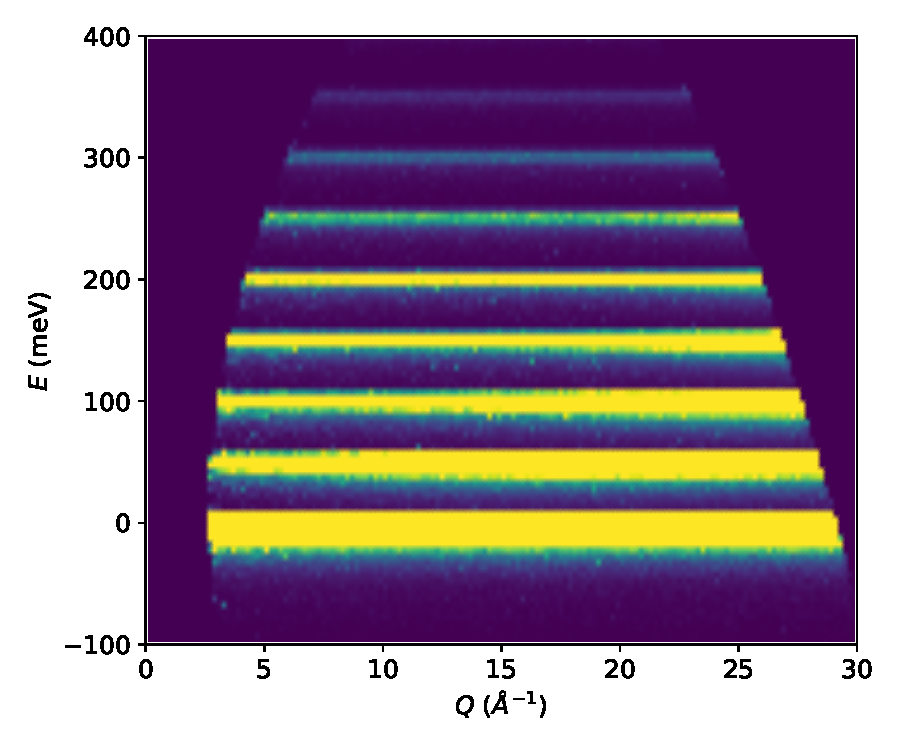
\includegraphics[width=\columnwidth]{figures/UN-ARCS-iqe.pdf}
\caption{The results from the UN simulation on ARCS with multiple scattering turned on. Color indicates the scattering intensity where brighter regions represent higher intensity. Note that the equally spaced lines are visible even at low $Q$.}
\label{fig:UN_plot}
\end{figure}

In this case, the incident beamline simulation (the simulation up to the sample containing the SNS source, guide choppers and slits) for the Wide Angular-Range Chopper Spectrometer (ARCS) instrument \cite{abernathy2012arcs, stone2014comparison} was run using McStas \cite{Willendrup:2020aa,Willendrup:2021aa} inside a workflow tool \cite{10.1007/978-3-031-23606-8_9}.
To configure the incident beam simulation in this workflow a user simply provides an existing experimental data file that provides the necessary parameters.
Specifically, an ARCS data file with an $E_i = 500$ meV was fed into the workflow which then generates an mcpl \cite{KITTELMANN201717} file \cite{data_doi} for use in MCViNE.
The rest of the virtual instrument uses \texttt{mcvine.acc} to leverage the GPU acceleration. It consists of a source component that reads the mcpl file to generate neutrons for the neutron source component,  a sample assembly component, and a powder $S(Q, E)$ monitor component for direct-geometry inelastic neutron spectrometers.
The results are shown in Figure~\ref{fig:UN_plot} and~\ref{fig:UN_cuts}.

First, note the equally spaced lines in $E$ shown in Figure~\ref{fig:UN_plot}. This the expected quantum oscillator behavior.
Furthermore, Figure~\ref{fig:UN_cuts} shows the $Q$ dependence of the scattering intensity along each of the $E$ lines in Figure~\ref{fig:UN_plot}.
The expected functional dependence for each successive transition and the overall increase in background expected from multiple scattering are both observed.

As this paper focuses on the GPU implementation, Figure~\ref{fig:UN_plot} and~\ref{fig:UN_cuts} also show the agreement between the CPU and GPU versions of MCViNE.
The majority of the speed increase for this particular simulation is in the incident beam line simulation leveraging the McStas GPU implementation, and is now under an hour rather than days.
The MCViNE part of the simulation has a speed up similar to the simpler test from $\sim 10^3$s to $\sim 10^2$s.
For a virtual neutron experiment the incident beam simulation can often be reused in a series of source-sample-detector simulations with various sample and detector configurations.
For example, a researcher may run the case with and without multiple scattering or a series of related samples. Thus fast sample simulations are critical to the overall speed of experimental analysis which highlights the need for using \texttt{mcvine.acc}.



\begin{figure}[h]
\centering
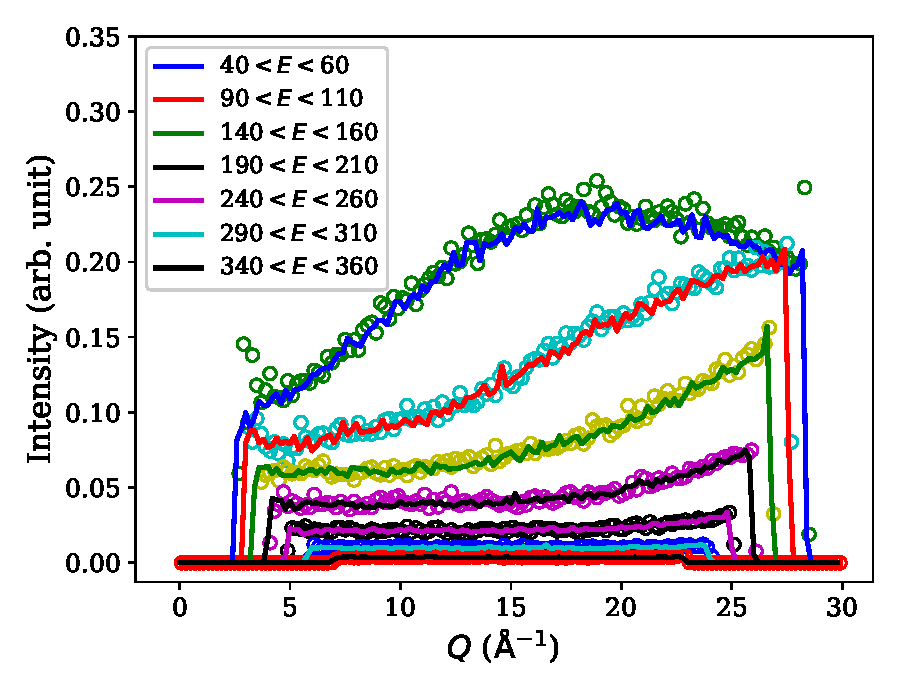
\includegraphics[width=\columnwidth]{figures/Constant_E_cuts_high_contrast.pdf}
\caption{Constant-$E$ cuts around the individual energy levels
in the $I(Q, E)$ displayed in
Figure~\ref{fig:UN_plot}. Note the functional dependence of each level and the background increase are consistent with the physics and the multiple scattering. The comparisons between the CPU and GPU calculations are shown with the solid line and circles respectively.
}
\label{fig:UN_cuts}
\end{figure}

\section{Conclusions}

Python and Numba were used successfully to create \texttt{mcvine.acc}, a new GPU accelerated version of MCViNE, which has so far achieved significant performance gains over the original CPU implementation. Using Python for this application has helped increase the usability, extensibility, and maintainability of the codebase, while gaining performance benefits of GPUs by using Numba. Additionally, the JIT nature of Numba allowed complex combinations of CUDA kernels to be generated at runtime, which would have been significantly harder to implement in other languages.

The performance gains from using Numba have shown to be beneficial. For a simple isotropic sphere sample, a speedup of 133x was achieved over a 16-core CPU using a consumer-grade GPU. For the more complex UN sample with multiple scattering, a speedup of 10x was achieved over a 16-core CPU. These performance gains are crucial for current simulations that take on the order of days to weeks to complete. However, there are still opportunities to further optimize these simulations to better leverage the full capability of the GPU.

Using Numba for GPU acceleration has enabled more sophisticated data analysis for neutron scattering and instrument design, while overall lowering the development cost needed to obtain significant performance improvements. The techniques used in this project could also be applied to other scientific computing applications.


\section{Acknowledgements}
For initial Framework development and instrument component development, this research used resources of the Spallation Neutron Source Second Target Station Project at Oak Ridge National Laboratory (ORNL). Sample development was sponsored by ORNL's Laboratory Director's Research and Development Fund. ORNL is managed by UT-Battelle LLC for DOE’s Office of Science, under Contract No. DE-AC05-00OR22725.

The US government retains and the publisher, by accepting the article for publication, acknowledges that the US government retains a nonexclusive, paid-up, irrevocable, worldwide license to publish or reproduce the published form of this manuscript, or allow others to do so, for US government purposes. DOE will provide public access to these results of federally sponsored research in accordance with the DOE Public Access Plan (\url{http://energy.gov/downloads/doe-public-access-plan}).
